\documentclass[a4paper,11pt]{report}

\usepackage{amsmath}
\usepackage{fullpage}
\usepackage{bussproofs}
\usepackage{mathpartir}
\usepackage{prooftrees}
\usepackage{color}

\usepackage{tikz}
\usetikzlibrary{automata,positioning}

\author{Sylvain Julmy}
\date{\today}

\setlength{\parindent}{0pt}

\newcommand*{\equal}{=}

\begin{document}

\begin{center}
  \large{
    Formal Methods\\
    Fall 2017
  }
  
  \noindent\makebox[\linewidth]{\rule{\linewidth}{0.4pt}}
  S05
  \noindent\makebox[\linewidth]{\rule{\linewidth}{0.4pt}}

  \begin{flushleft}
    Professor : Ultes-Nitsche Ulrich

    Assistant : Christophe Stammet
  \end{flushleft}

  
  \noindent\makebox[\linewidth]{\rule{\linewidth}{0.4pt}}

  Submitted by Sylvain Julmy
  
  \noindent\makebox[\linewidth]{\rule{\textwidth}{1pt}}
\end{center}

\section*{Exercise 1}

\subsection*{(1)}

We assume that the language is on the right of the Turing Machine tape.

\begin{center}
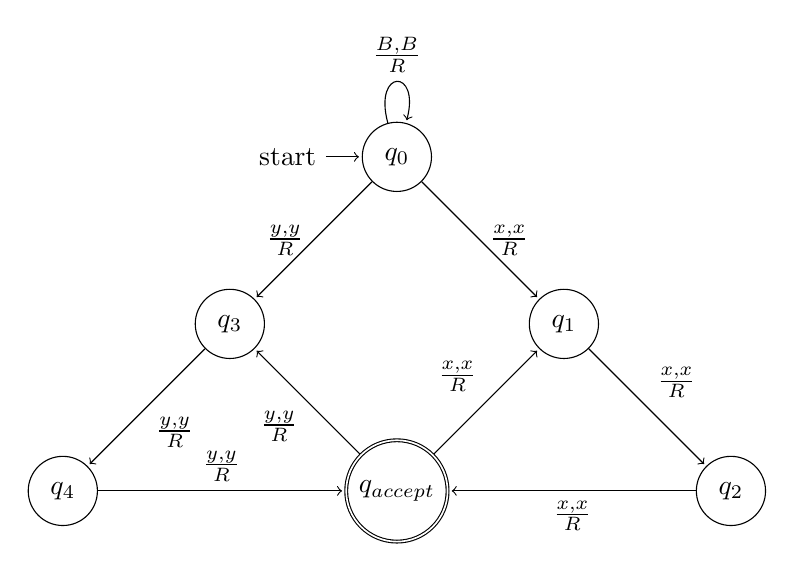
\begin{tikzpicture}[shorten >=1pt,node distance=3cm,on grid,auto]
\node[state,initial] (q0) {$q_0$};
\node[state] (q1) [below right = of q0] {$q_1$};
\node[state] (q2) [below right = of q1] {$q_2$};
\node[state] (q3) [below  left= of q0] {$q_3$};
\node[state] (q4) [below left = of q3] {$q_4$};
\node[state,accepting] (qa) [below left = of q1] {$q_{accept}$};
\path[->]
(q0)
edge [loop above] node {$\frac{B,B}{R}$} ()
edge [] node [right] {$\frac{x,x}{R}$} (q1)
edge [] node [left] {$\frac{y,y}{R}$} (q3)
(q1)
edge [] node [] {$\frac{x,x}{R}$} (q2)
(q2)
edge [] node [] {$\frac{x,x}{R}$} (qa)
(q3)
edge [] node [] {$\frac{y,y}{R}$} (q4)
(q4)
edge [] node [] {$\frac{y,y}{R}$} (qa)
(qa)
edge [] node [] {$\frac{x,x}{R}$} (q1)
edge [] node [] {$\frac{y,y}{R}$} (q3)
;
\end{tikzpicture}
\end{center}

\subsection*{(2)}

\begin{center}
\begin{tikzpicture}[shorten >=1pt,node distance=3cm,on grid,auto]
\node[state,initial] (q0) {$q_0$};
\node[state] (q1) [below left = of q0] {$q_1$};
\node[state] (q2) [right = of q1] {$q_2$};
\node[state] (q3) [right = of q2] {$q_3$};
\node[state] (qn) [right = of q3] {$q_{notAccept}$};
\node[state] (qb) [below = of q3] {$q_{back}$};
\node[state] (qsw) [below = of qb] {$q_{startWrite}$};
\node[state] (q4) [left = of qsw] {$q_4$};
\node[state,accepting] (qe) [left = of q4] {$q_{end}$};
\path[->]
(q0)
edge [loop above] node [] {$\frac{B,B}{R}$} ()
edge [] node [] {$\frac{y,y}{R}$} (q1)
edge [] node [] {$\frac{x,x}{R}$} (q2)
(q1)
edge [loop left] node [] {$\frac{y,y}{R}$} ()
edge [] node [below] {$\frac{x,x}{R}$} (q2)
(q2)
edge [] node [below] {$\frac{x,x}{R}$} (q3)
edge [loop below] node [] {$\frac{y,y}{R}$} ()
(q3)
edge [loop above] node [] {$\frac{y,y}{R}$} ()
edge [] node [below] {$\frac{x,x}{R}$} (qn)
edge [] node [] {$\frac{B,B}{L}$} (qb)
(qb)
edge [loop left] node [] {$\frac{y,y}{L}$} ()
edge [loop right] node [] {$\frac{x,x}{L}$} ()
edge [] node [] {$\frac{B,B}{R}$} (qsw)
(qsw)
edge [loop right] node [] {$\frac{y,B}{R}$} ()
edge [loop below] node [] {$\frac{x,B}{R}$} ()
edge [] node [] {$\frac{B,x}{R}$} (q4)
(q4)
edge [] node [] {$\frac{B,x}{R}$} (qe)
;
\end{tikzpicture}
\end{center}

\section*{Exercise 2}

In order to prove the non-computability of the Busy Beaver function, we can use
the following steps :

\begin{itemize}
\item Generate every Turing machine with $n$ states, there is a finite number of
  these.
\item For each machine, we run it and count out the number of $1$ on the tape
  when the machine halt.
\end{itemize}

The problem is that we don't know which of the machine goes forever or not, and
that is the halting problem solve in previous exercises sheet.

The other way is to use the statement from the exercice. If $a > b$, $BB(a)$
would always be greater than $BB(b)$. We imagine we have a Busy Beaver TM with
$n$ states, independently of the output of $BB(n)$, the Busy Beaver TM with
$n+1$ states could always write at least $1$ more $1$ on the tape by simply
adding a state to $TM_{BB}(n)$ which simply write an $1$ and stop in an
accepting state. So the $BB(n)$ function is strictly increasing.

\section*{Exercise 3}

\subsection*{(1)}
Given a Turing Machine $M$ that decide the recursive language $L$, we can
create the Turing Machine that decide $\overline{L}$ : On input $x$, run $M$ on
$x$. Then, $x$ is accepted if $M$ rejects $x$ and $x$ is rejected if $M$ accepts
$x$. So we have construct the Turing Machine for $\overline{L}$, which stop in
an accepting state where $w \in \overline{L}$ and stop in an non-accepting state
where $w \not\in \overline{L}$.

\subsection*{(2)}

Recursive language are closed under the union.

\begin{proof}
Given two Turing Machine $M_1$ and $M_2$ which are accepting $L_1$ and
respectivly $L_2$, we construct the Turing machine that decide $L_1 \cup L_2$ :
on input $x$, run $M_1$ and $M_2$, add accept $x$ only if and only if $M_1$ or
$M_2$ accept $x$.
\end{proof}

Recursive language are closed under the intersection.

\begin{proof}
Given two Turing Machine $M_1$ and $M_2$ which are accepting $L_1$ and
respectivly $L_2$, we construct the Turing machine that decide $L_1 \cap L_2$ :
on input $x$, run $M_1$ and $M_2$, add accept $x$ only if and only if $M_1$ and
$M_2$ accept $x$.
\end{proof}


\end{document}

%%% Local Variables:
%%% mode: latex
%%% End:
